\section{Overall Research Plan}
\label{sec:overallresearchplan}

To the best of our knowledge there are not, out there, OpenMP data race
detectors that guarantee low runtime and memory overhead while maintaining
high precision and accuracy.
%
This motivates the need for better data race detection techniques and tools
for structured parallel programming paradigms.
%
As claimed in \S~\ref{sec:introduction}, we propose several different
contributions to obtain a faster data race detection tool for large OpenMP
programs.
%
In the remainder of this section I will discuss and detail our proposed
contributions and how the combination of them helps to obtain a better OpenMP
data race detector.

\textbf{Sequential Blacklisting:} We exploit OpenMP's structured parallelism
to identify guaranteed sequential regions within OpenMP code.
%
Such analysis would be difficult to conduct in the context of unstructured
parallelism (e.g., PThreads).
%
Figure~\ref{fig:nested} shows an example of OpenMP parallel and nested
parallel regions.
%
As we can see, the parallel regions are alternated by the solely main thread
execution.
%
The code executed by the main thread is sequential and cannot race with any
other threads existing in a parallel region.
%
Therefore, the instructions executed by the main thread during its sequential
execution can be excluded from the runtime analysis reducing the overhead.

\begin{figure}
  \centering
  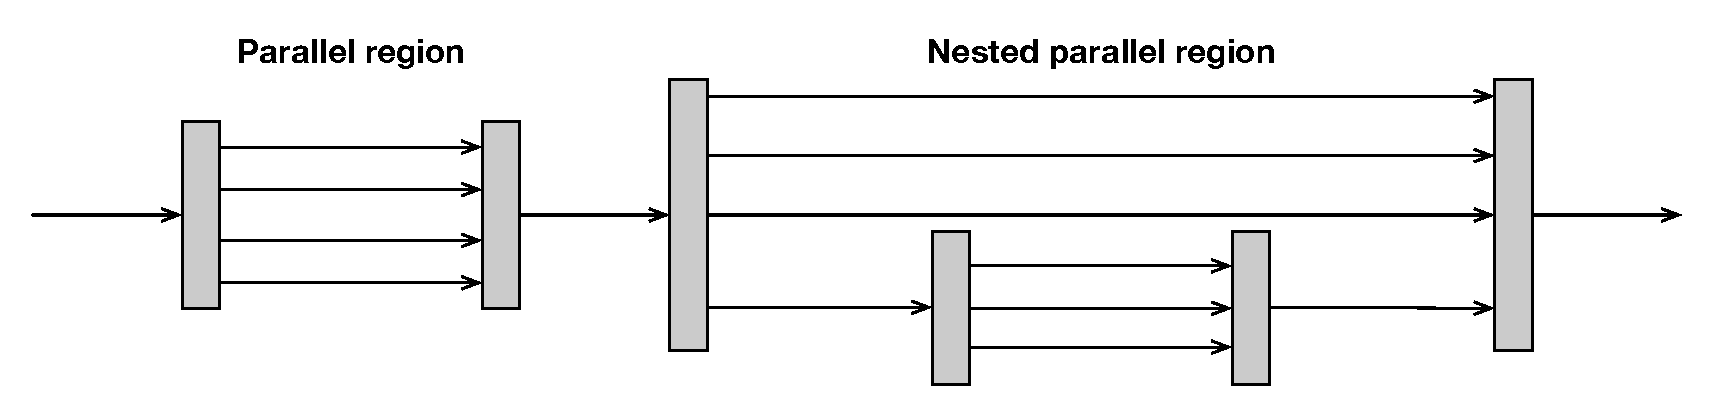
\includegraphics[width=0.95\textwidth]{figures/nested_parallelism}
  \caption{OpenMP nested parallelism}
  \label{fig:nested}
\end{figure}

\textbf{Data Dependency Analysis:} We identify and suppress race free parallel
loops from race checking.
%
Listing~\ref{code:example01} shows an example of two parallel for-loops.
%
The first one is easily and automatically parallelizable, the array will be
divided in different chunks and each of them will be assigned to different
threads.
%
However, the second parallel for-loops has a data dependency in the array
accesses, which will introduce a data race when the array's chunks are
assigned to different threads.
%
Indeed, it may happen that two threads will access the same locations
simultaneously without any synchronization mechanism.
%
The OpenMP compiler do not apply any check and will parallelize both loop in
the same way.
%
We introduce a data dependency analysis at compiling time that identify loops
with and without dependencies.
%
The firsts will be blacklisted and excluded by the runtime analysis since race
free, the seconds instead will be checked at runtime.

\begin{wrapfigure}{L}{0.37\textwidth}
  \vspace{-2ex}
  \begin{lstlisting}[language=C++, caption=OpenMP loops with and without loop-carried data dependency., label=code:example01]
  #pragma omp parallel for
  for(int i = 0; i < N; i++) {
    a[i] = a[i] + 1;
  }

  #pragma omp parallel for
  for(int i = 1; i < N; i++) {
    a[i] = a[i - 1];
  }
  \end{lstlisting}
\end{wrapfigure}

\textbf{\archer v1:} The two previous static analysis techniques and an
instrumented version of the OpenMP runtime make the first version of the
OpenMP data race detector \archer.
%
The static analyses will be implemented as a LLVM/Clang passes and integrated
in the compilation process.
%
We will annotate the OpenMP runtime to communicate the \tsan about the
happens-before relations between threads in presence of unknown
synchronization mechanisms.
%
For example, OpenMP barriers and OpenMP critical section are unknown to the
\tsan runtime, which would make it reports false positives.
%
This first version of \archer is the initial step towards low overhead data
race detector for large OpenMP applications, and it would also allow us to
evaluate the benefits of the static analyses in terms of both overheads
reduction, and precision and accuracy of the data race detection process.

\textbf{Clock-less runtime algorithm:} We propose a new data race detection
algorithm that, differently from past and modern Pthreads data race detection
techniques usually based on vector and lamport clocks, exploits the structured
parallelism of parallel programming models, such as OpenMP, and a fast data
structure to maintain much less state and/or traverse much less code paths.
%
Our approach consists in a pre-pass data race detection that quickly
identifies at runtime possible memory conflicts.
%
The result may contain both real races and false positives.
%
Therefore we also implement an infrastructure to double check the result with
a slower but more precise data race detection tool (i.e. Tsan) to identify the
real races from the false positives.

The goal is to rapidly identify possible memory conflicts in very large OpenMP
applications without the need of enormous amount of resources (runtime and
memory), which often are not available.
%
The user can decide to analyze manually the result of the race detection
pre-pass, and/or if necessary run the program again and analyze it with a more
precise race detection technique.
%
The second-pass analysis will only analyze the memory conflicts reported by
the pre-pass analysis, in this way we can speedup the analysis process of
slower data race detection techniques.
%
Furthermore, the second-pass analysis will not require any further action from
the user besides normally execute the program again.

In order to design and implement a low overhead data race detection technique
we plan to use probabilistic data structures such as Bloom
Filters~\cite{Bloom:1970:STH:362686.362692}.
%
A bloom filter enables inserting elements in a set and test whether an element
belongs this set, sacrificing accuracy for lower memory usage.
%
More precisely, it can say an element is in the set when in it’s not (false
positive), but if it says it’s not in the set, then it’s true (no false
negatives).
%
In a nutshell, we use such a data structure to store the memory accesses
performed by threads, and check if a new memory access belong to this set, if
that's the case we find a memory conflict.
%
Obviously the mechanism is not that simple.
%
In order to identify if a memory conflict is a real race or not we need to
consider several scenarios.
%
A data race happens when two different threads access the same memory
location, at least on of them is performing a write operation, and the access
is not synchronized (i.e. atomic, mutex).
%
Only checking if a memory location has been already accessed by a thread is
not enough.
%
Our technique maintains different filters to discriminate the different
scenarios, for example we have a filter for unprotected reads, a filter for
unprotected writes, and so on for atomic and critical section protected
operations.

A classic bloom filter would not allow to identify if a memory access has been
performed by a different or same thread, since we can only ``store'' the
memory location.
%
Therefore we actually improve our approach using the bloom filter as a
key-store value in order to store the last thread id that accessed the memory
location.
%
In literature there have been many attempts of using bloom filters for
key-store~\cite{6995996} value or for counting how many times a certain
element has been inserted in the set~\cite{Deng:2006:ADD:1142473.1142477}.
%
Our intent is to adopt one of these bloom-filter alternatives to sore the
thread it of a certain memory access and increase the precision and accuracy
of data race detection algorithm.
%
We will study the different data structures to identify the best fit for our
purposes, and if necessary modify existing solutions for optimal results.

\textbf{\archer v2:} The second version of \archer will embed both static
analyses and the fast runtime analysis technique for data race detection.
%
We plan to integrate \archer in the LLVM/Clang compiler infrastructure and
guarantee the same ease to use that characterize most LLVM tools.
%
In fact, we will provide a new compilation flag (i.e. ``-archer'') that will
instrument the OpenMP program at compile time and will link it against the
\archer runtime library.
%
The program can then be executed as usual, while the \archer runtime library
will perform the data race detection providing at the end of the execution a
detailed report about the detected races.

%%% Local Variables:
%%% mode: latex
%%% eval: (flyspell-mode 1)
%%% TeX-master: "root.tex"
%%% End:
